% ============================================================
% Revised Methodology — Based on Actual Implementation & Results
% ============================================================
% Drop this into your main paper .tex, replacing the old \section{Proposed Methodology}
% Figures referenced here should be placed in a figures/ directory
% or adjust paths as needed.

\section{Methodology}
\label{sec:methodology}

To address the brittleness of single-modality geometric descriptors, particularly under adverse weather conditions, we frame Loop Closure Detection (LCD) as a multi-modal metric learning problem. Our approach leverages a supervised deep learning pipeline to fuse high-dimensional LiDAR scans and RGB camera feeds into a compact, rotation-invariant latent space.

The overall architecture operates on a ``student-teacher'' paradigm. The robot's fused raw sensor data acts as the input to the student network (the multi-modal CNN), while the absolute global positioning system (GPS) acts as the teacher, providing the strict supervisory signal required to mine training triplets and penalize incorrect loop closures.

\subsection{Dataset \& Time Synchronization}
We utilize a proprietary 500+ GB dataset collected specifically for this research on the North Carolina A\&T State University campus (Fig.~\ref{fig:trajectory}).
\begin{itemize}
    \item \emph{Spatial Sensor:} Ouster OS1-128 LiDAR (10~Hz), providing high-density 128-beam 3D point clouds.
    \item \emph{Visual Sensor:} Forward-facing USB RGB Camera (30~Hz).
    \item \emph{Ground Truth (Teacher):} NovAtel SPAN GNSS/INS (OEM7), providing centimeter-level global positioning data.
\end{itemize}

A fundamental engineering challenge in sensor fusion is asynchronous data rates. Because the camera operates at 3$\times$ the frequency of the LiDAR, naive sequential pairing is impossible. In our pre-processing pipeline, we employ an Approximate Time Synchronizer to match the closest camera frame to each LiDAR sweep within a rigid 50~ms tolerance. This yields approximately 14,000 time-synchronized sensor pairs that are split chronologically into 70\% training, 15\% validation, and 15\% test sets.

\begin{figure}[t]
    \centering
    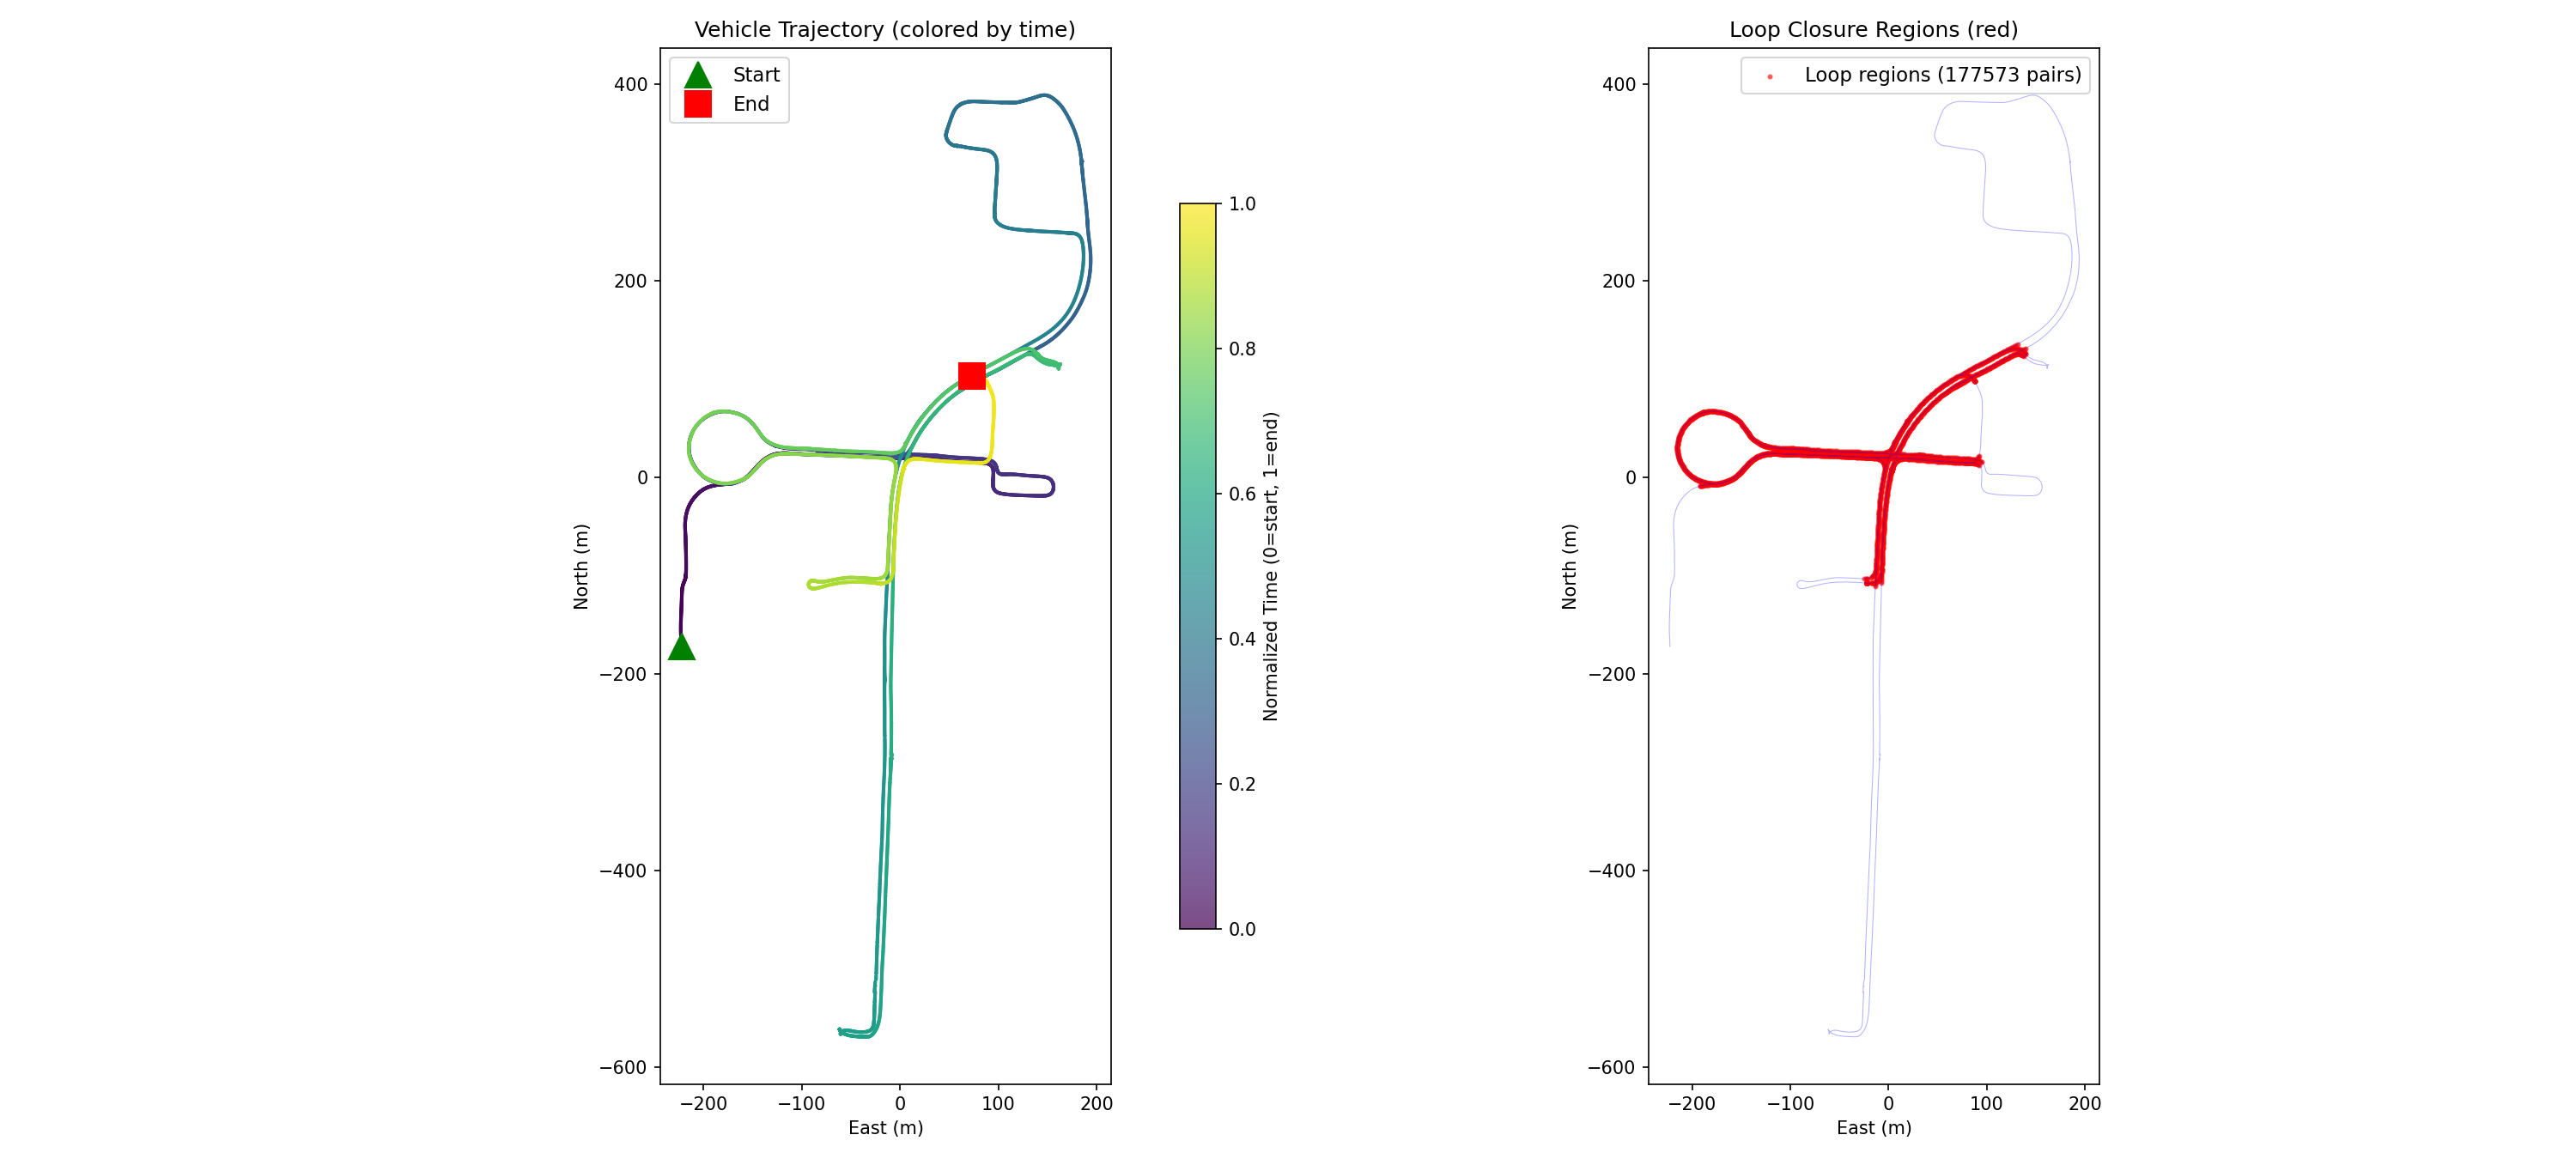
\includegraphics[width=\linewidth]{figures/trajectory.png}
    \caption{Vehicle trajectory on the NC A\&T campus (left), colored by normalized time. Loop closure regions where the vehicle revisits the same location are highlighted in red (right), totaling 177{,}573 positive pairs.}
    \label{fig:trajectory}
\end{figure}

\subsection{Spatial Data Representation (Range Images)}
Processing unstructured 3D point clouds directly via neural networks is computationally prohibitive for real-time edge deployment. To bridge this gap, we project each 3D LiDAR point cloud into a dense 2D spherical projection, known as a \emph{Range Image} (Fig.~\ref{fig:sample_pairs}).

For a given 3D point $P = (x, y, z)$, the corresponding pixel value $r$ in the range image is calculated as the Euclidean distance from the sensor origin:
\begin{equation}
    I(u, v) = r = \sqrt{x^2 + y^2 + z^2}
\end{equation}
This transformation converts the sparse 3D data into a dense image tensor of size $128 \times 1024$, exploiting the full vertical resolution of the 128-beam sensor. This allows us to leverage highly optimized standard 2D CNNs for spatial feature extraction.

\begin{figure}[t]
    \centering
    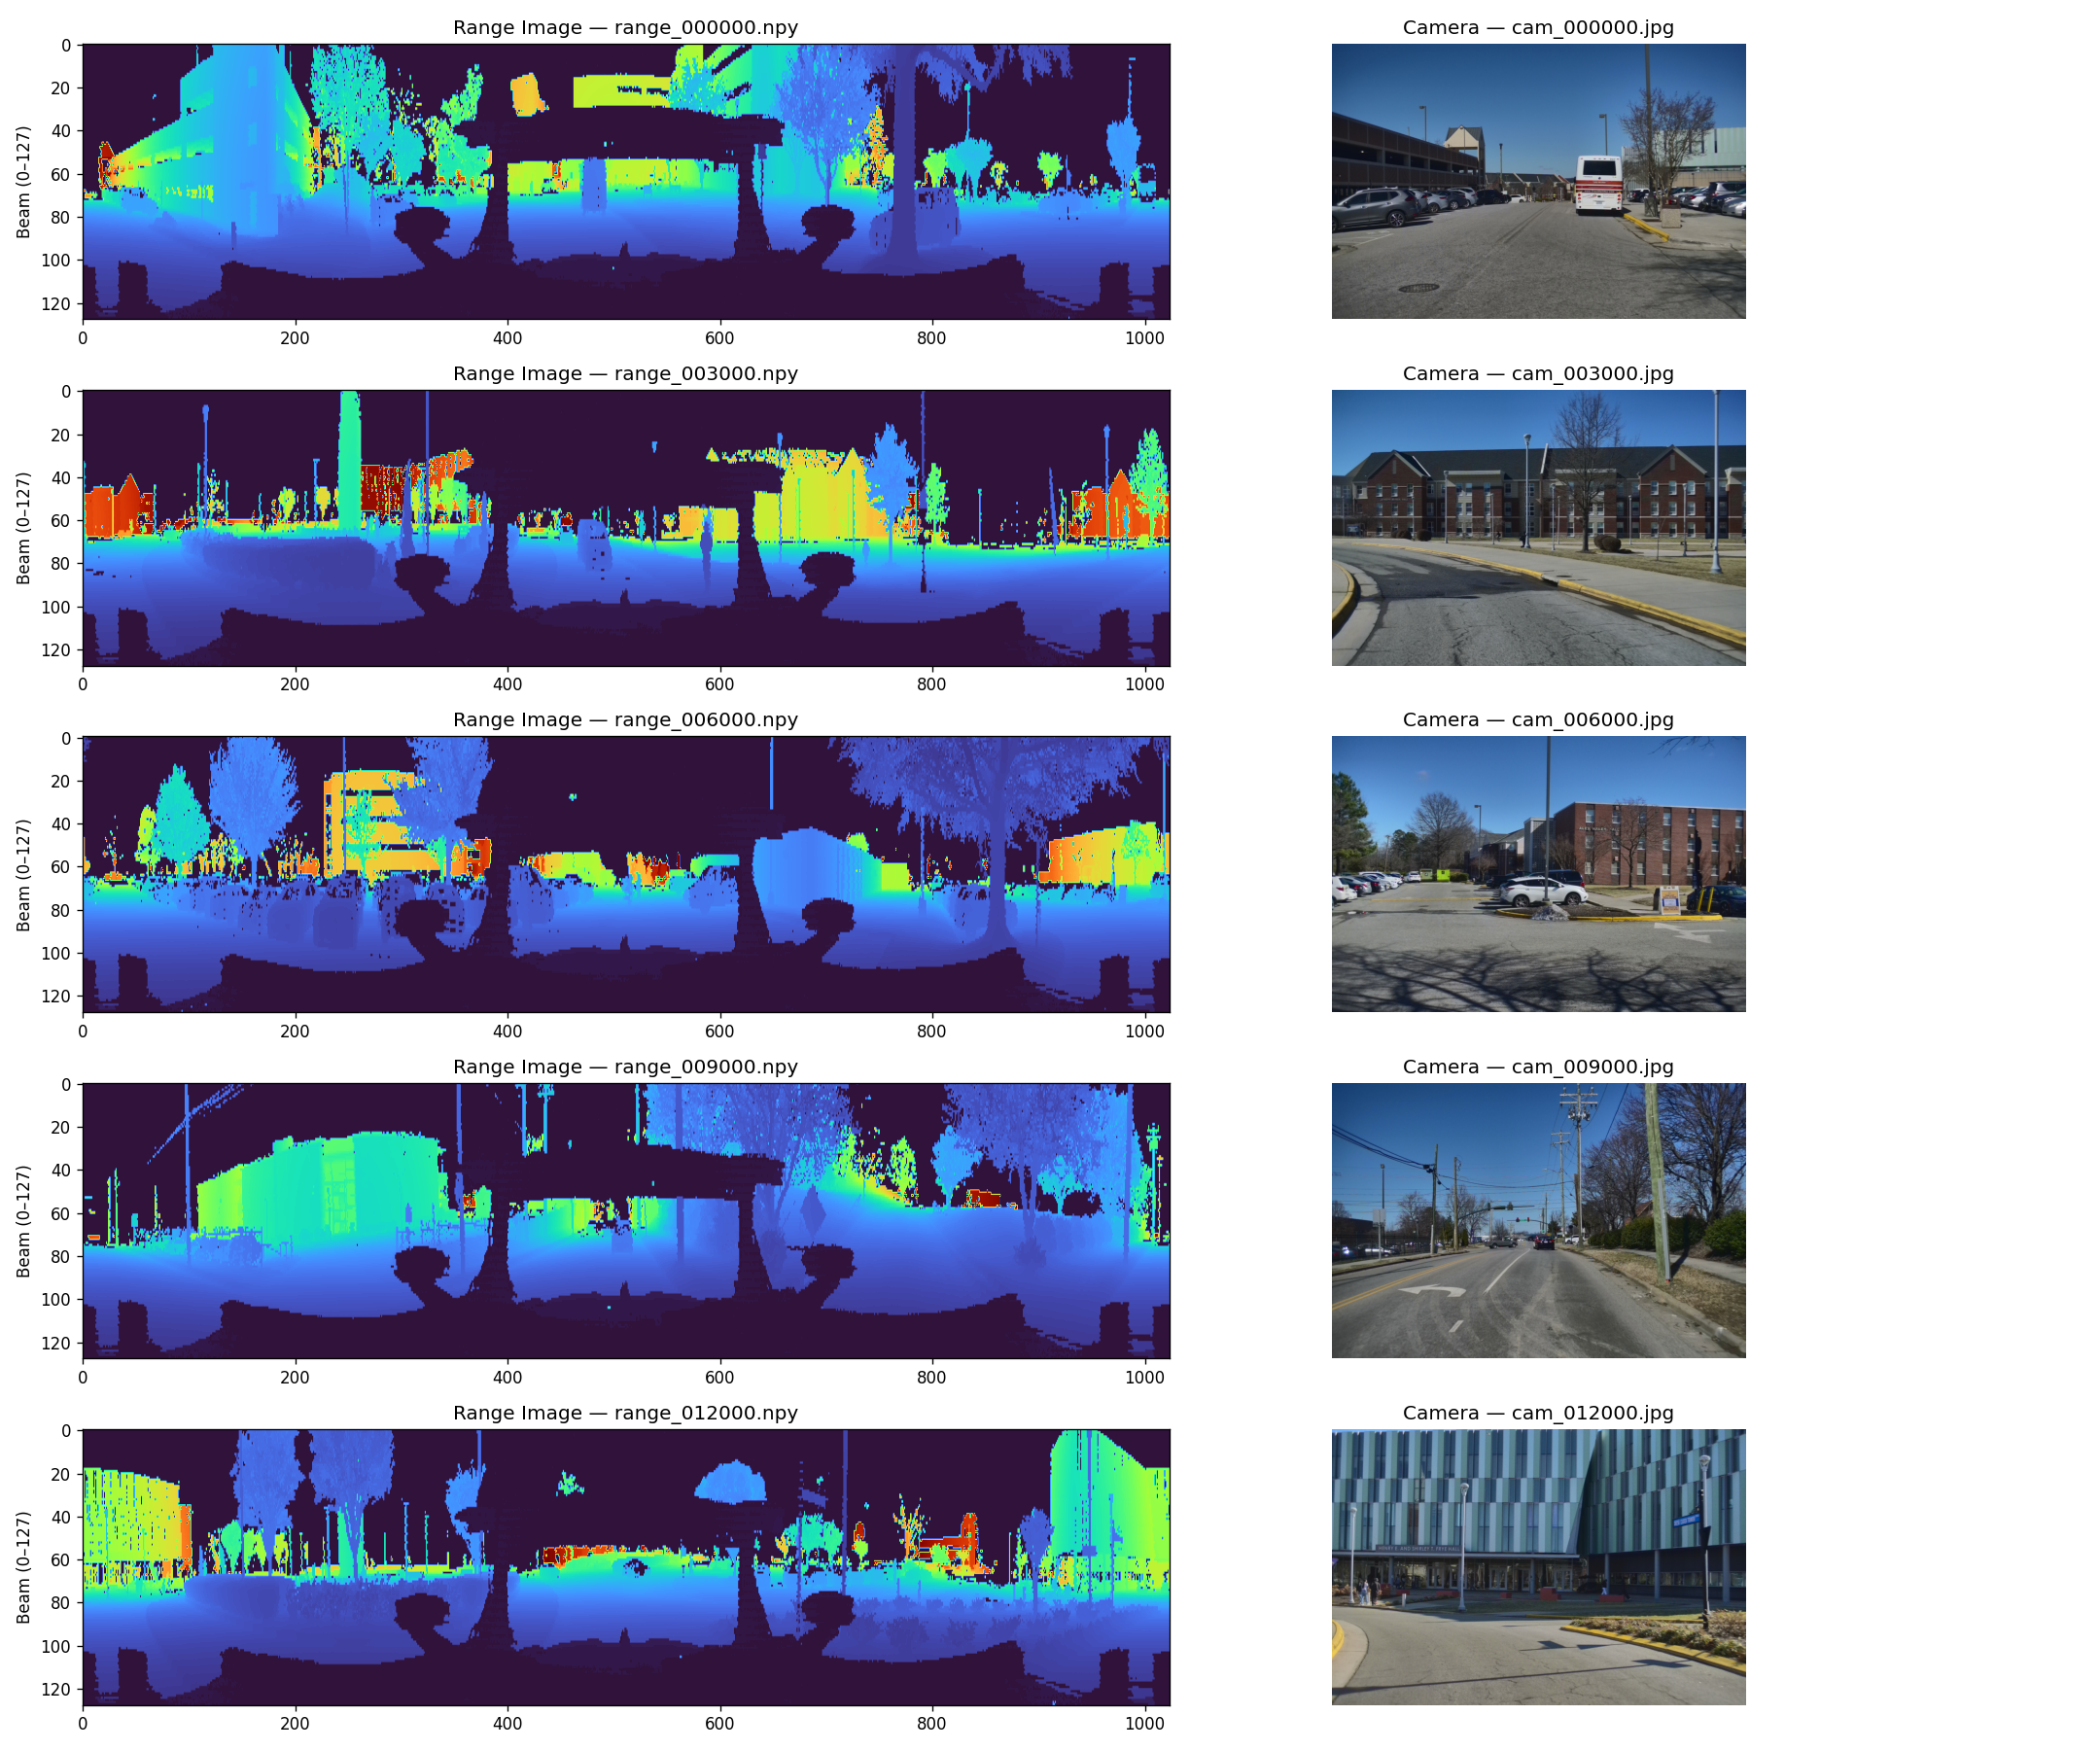
\includegraphics[width=\linewidth]{figures/sample_pairs.png}
    \caption{Time-synchronized sensor pairs used for training. Each row shows a LiDAR range image (left) alongside its corresponding camera frame (right). The range images encode depth information as a color map, preserving 3D structural geometry in a dense 2D representation.}
    \label{fig:sample_pairs}
\end{figure}

\subsection{Two-Stream Siamese Network Architecture}
The core of our feature extraction pipeline is a \emph{Two-Stream Siamese Neural Network}. Unlike standard classifiers that output a discrete probability, this network learns a fused similarity metric in the embedding space. The architecture is illustrated in Fig.~\ref{fig:architecture}.

The encoder consists of two parallel branches:
\begin{enumerate}
    \item \textbf{LiDAR Stream:} A ResNet-18 backbone, modified with a single-channel input convolution (initialized from the mean of pretrained RGB filters), processes the $128 \times 1024$ range image and produces a 512-d feature vector.
    \item \textbf{Camera Stream:} A standard pretrained ResNet-18 backbone processes the $224 \times 224$ RGB image, also producing a 512-d feature vector.
\end{enumerate}

The outputs of these two streams are concatenated into a 1024-d vector and passed through a fusion MLP: a fully-connected layer ($1024 \rightarrow 512$), followed by Batch Normalization, ReLU, Dropout ($p{=}0.1$), and a final linear projection to 256 dimensions. The output is L2-normalized to produce a unit-length ``location fingerprint.'' The total model contains approximately 23 million trainable parameters.

\begin{figure}[t]
    \centering
    \begin{tikzpicture}[
        node distance=0.8cm,
        block/.style={rectangle, draw, fill=blue!10, text width=2.8cm, text centered, minimum height=0.7cm, font=\small},
        input/.style={rectangle, draw, fill=green!10, text width=2.5cm, text centered, minimum height=0.7cm, font=\small},
        output/.style={rectangle, draw, fill=red!10, text width=3cm, text centered, minimum height=0.7cm, font=\small},
        arrow/.style={->, thick}
    ]
    % Inputs
    \node[input] (lidar) {LiDAR Range Image\\$(1, 128, 1024)$};
    \node[input, right=2.5cm of lidar] (camera) {Camera RGB\\$(3, 224, 224)$};
    
    % Backbones
    \node[block, below=of lidar] (resnet_l) {ResNet-18\\(modified)};
    \node[block, below=of camera] (resnet_c) {ResNet-18\\(pretrained)};
    
    % Feature vectors
    \node[block, below=of resnet_l] (feat_l) {512-d features};
    \node[block, below=of resnet_c] (feat_c) {512-d features};
    
    % Concat
    \node[block, below right=0.8cm and -0.7cm of feat_l, text width=3.5cm, fill=orange!15] (concat) {Concatenate\\1024-d};
    
    % Fusion
    \node[block, below=of concat, fill=purple!10, text width=4cm] (fusion) {Fusion MLP\\$1024 \rightarrow 512 \rightarrow 256$};
    
    % Output
    \node[output, below=of fusion] (desc) {256-d L2-normalized\\Location Fingerprint};
    
    % Arrows
    \draw[arrow] (lidar) -- (resnet_l);
    \draw[arrow] (camera) -- (resnet_c);
    \draw[arrow] (resnet_l) -- (feat_l);
    \draw[arrow] (resnet_c) -- (feat_c);
    \draw[arrow] (feat_l) -- (concat);
    \draw[arrow] (feat_c) -- (concat);
    \draw[arrow] (concat) -- (fusion);
    \draw[arrow] (fusion) -- (desc);
    \end{tikzpicture}
    \caption{Two-Stream Encoder architecture. The LiDAR and camera streams are processed by parallel ResNet-18 backbones, concatenated, and compressed through a fusion MLP into a compact 256-d descriptor.}
    \label{fig:architecture}
\end{figure}

\subsubsection{Modality Dropout}
To encourage robustness when one sensor is degraded (e.g., camera blinded by glare, or LiDAR returns corrupted by rain), we employ \emph{modality dropout} during training. With probability $p_{\text{drop}}{=}0.15$, one of the two 512-d feature vectors is zeroed out \emph{after} the backbone but \emph{before} the fusion MLP. This forces the network to learn representations that are informative from either modality independently, rather than relying on a fixed combination.

\subsection{Training Strategy}
\subsubsection{GPS-Supervised Triplet Mining}
Using the GPS ground truth as the supervisory signal, we mine training triplets offline. For each anchor frame at position $\mathbf{x}_a$, we select:
\begin{itemize}
    \item A \emph{positive} frame at position $\mathbf{x}_p$ such that $\|\mathbf{x}_a - \mathbf{x}_p\| < d_{\text{pos}}$ and $|t_a - t_p| > d_{\text{time}}$, ensuring it is the same location but at a different time.
    \item A \emph{negative} frame at position $\mathbf{x}_n$ such that $\|\mathbf{x}_a - \mathbf{x}_n\| > d_{\text{neg}}$, from a geographically distinct area.
\end{itemize}
We set $d_{\text{pos}} = 5$~m, $d_{\text{neg}} = 25$~m, and $d_{\text{time}} = 60$~s. This produces 22{,}807 training triplets and 9{,}912 validation triplets.

\subsubsection{Triplet Margin Loss}
The network is optimized using Triplet Margin Loss with margin $\alpha = 1.0$:
\begin{equation}
    \mathcal{L} = \max\left(\|f(A) - f(P)\|_2 - \|f(A) - f(N)\|_2 + \alpha,\; 0\right)
\end{equation}
where $f(\cdot)$ denotes the encoder output. The three triplet branches share identical weights—we define one encoder and call it three times. The anchor, positive, and negative inputs are concatenated into a single batch and forwarded together, ensuring stable Batch Normalization statistics.

\subsubsection{Two-Phase Training with Online Hard Mining}
We observe that randomly-mined negatives become trivially easy after a few epochs, causing the loss to collapse to near-zero while the model fails to distinguish genuinely confusable locations. To address this, we implement a \emph{two-phase training strategy} (Fig.~\ref{fig:training_curves}):

\textbf{Phase~1 (Triplet Pre-training):} The model trains on the full set of 22{,}807 mined triplets using Adam optimizer ($\text{lr}{=}10^{-4}$, weight decay $10^{-5}$), with automatic mixed precision (AMP) and gradient accumulation (effective batch size 48). Training proceeds until early stopping (patience = 10 epochs). This phase establishes broad spatial representations across the entire route.

\textbf{Phase~2 (Hard Mining Fine-tuning):} Using the GPS coordinates, we partition training frames into 95 discrete geographic ``places'' via spatial grid quantization ($5\text{m} \times 5\text{m}$ cells), retaining only cells with genuine revisits ($\Delta t > 60$~s). We then employ a PK batch sampler that constructs batches of $P{=}8$ places $\times$ $K{=}4$ frames per place. Within each batch, we compute \emph{batch-hard triplet loss}: for each anchor, we find the hardest positive (same place, maximum distance) and hardest negative (different place, minimum distance):
\begin{equation}
    \mathcal{L}_{\text{hard}} = \frac{1}{|B|}\sum_{i \in B} \max\left(\max_{j: y_j = y_i} d_{ij} - \min_{k: y_k \neq y_i} d_{ik} + \alpha,\; 0\right)
\end{equation}
This phase fine-tunes at $0.1\times$ the Phase~1 learning rate for up to 20 epochs.

\begin{figure}[t]
    \centering
    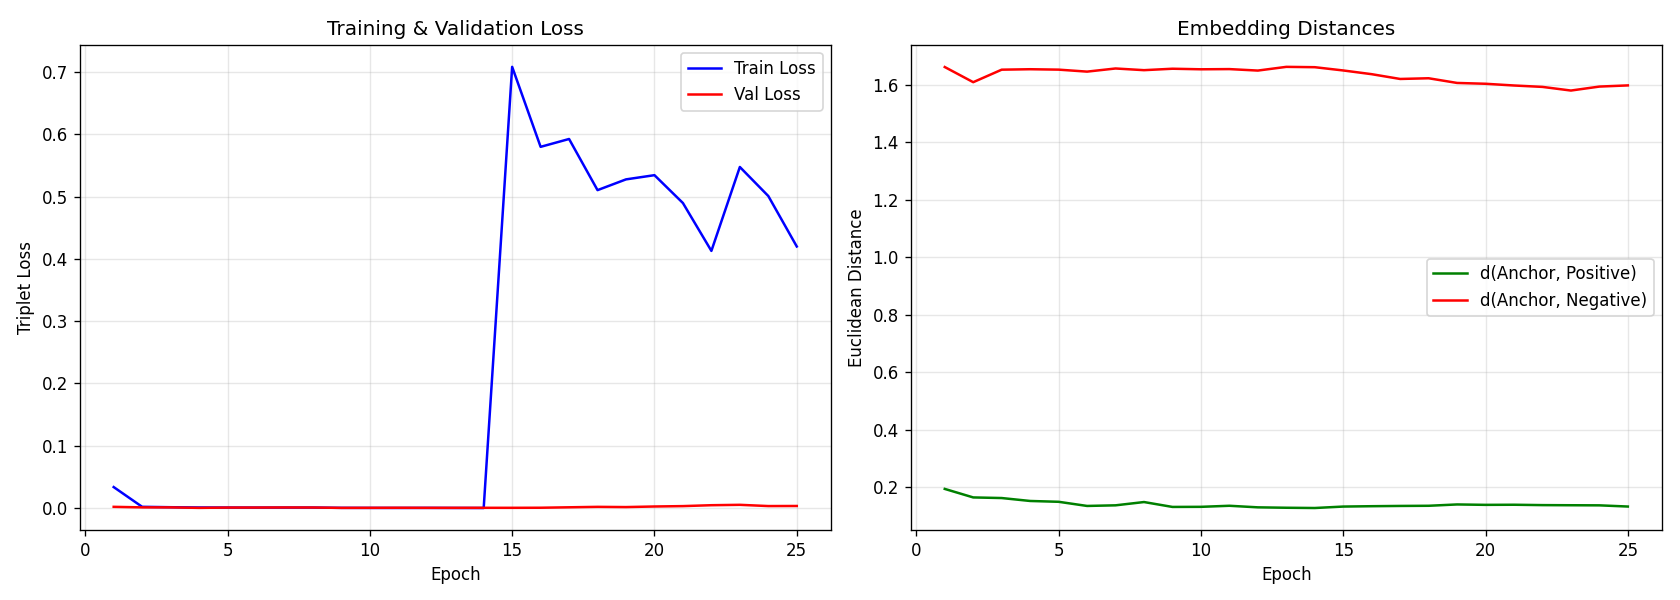
\includegraphics[width=\linewidth]{figures/training_curves.png}
    \caption{Two-phase training dynamics. Phase~1 (epochs 1--14) uses pre-mined triplets; loss converges near zero as random negatives become trivial. Phase~2 (epochs 15--25) switches to online batch-hard mining; training loss spikes to ${\sim}0.7$ as the model confronts genuinely confusable frame pairs, then gradually decreases. Embedding distances (right) show the positive distance $d(A,P)$ decreasing and the negative distance $d(A,N)$ remaining well-separated throughout.}
    \label{fig:training_curves}
\end{figure}

\subsubsection{Data Augmentation}
To improve generalization and simulate sensor degradation, we apply stochastic augmentations during training:
\begin{itemize}
    \item \emph{Camera:} Random color jitter (brightness, contrast, saturation, hue), random horizontal flip, and standard ImageNet normalization.
    \item \emph{LiDAR:} Additive Gaussian noise ($\sigma{=}0.02$) and random rectangular patch dropout (up to 10\% of the range image zeroed), simulating sensor noise and occlusions.
\end{itemize}

\section{Preliminary Results}
\label{sec:results}

We evaluate the trained model on 2{,}000 held-out test frames (15\% chronological split), computing pairwise descriptor distances across all $\binom{2000}{2} \approx 2$~million frame pairs. A pair is considered a true positive if $\|\mathbf{x}_i - \mathbf{x}_j\| < 5$~m and $|t_i - t_j| > 60$~s, yielding 6{,}455 positive pairs.

\subsection{Quantitative Results}

Table~\ref{tab:results} summarizes the performance across three descriptor modes: the full fused model, LiDAR-only (camera features zeroed), and camera-only (LiDAR features zeroed). The Precision-Recall curves are shown in Fig.~\ref{fig:pr_curves}.

\begin{table}[t]
\centering
\caption{Loop closure detection performance on the test set (2{,}000 frames, 6{,}455 positive pairs).}
\label{tab:results}
\begin{tabular}{lccc}
\toprule
\textbf{Metric} & \textbf{Fused} & \textbf{LiDAR-only} & \textbf{Camera-only} \\
\midrule
AUC-PR       & \textbf{0.1562} & 0.1398 & 0.1165 \\
F1-max       & \textbf{0.2675} & 0.2218 & 0.2106 \\
Recall@1     & 0.1583 & \textbf{0.1864} & 0.1142 \\
Best Thresh. & 0.9932 & 0.9850 & 0.9910 \\
\bottomrule
\end{tabular}
\end{table}

\begin{figure}[t]
    \centering
    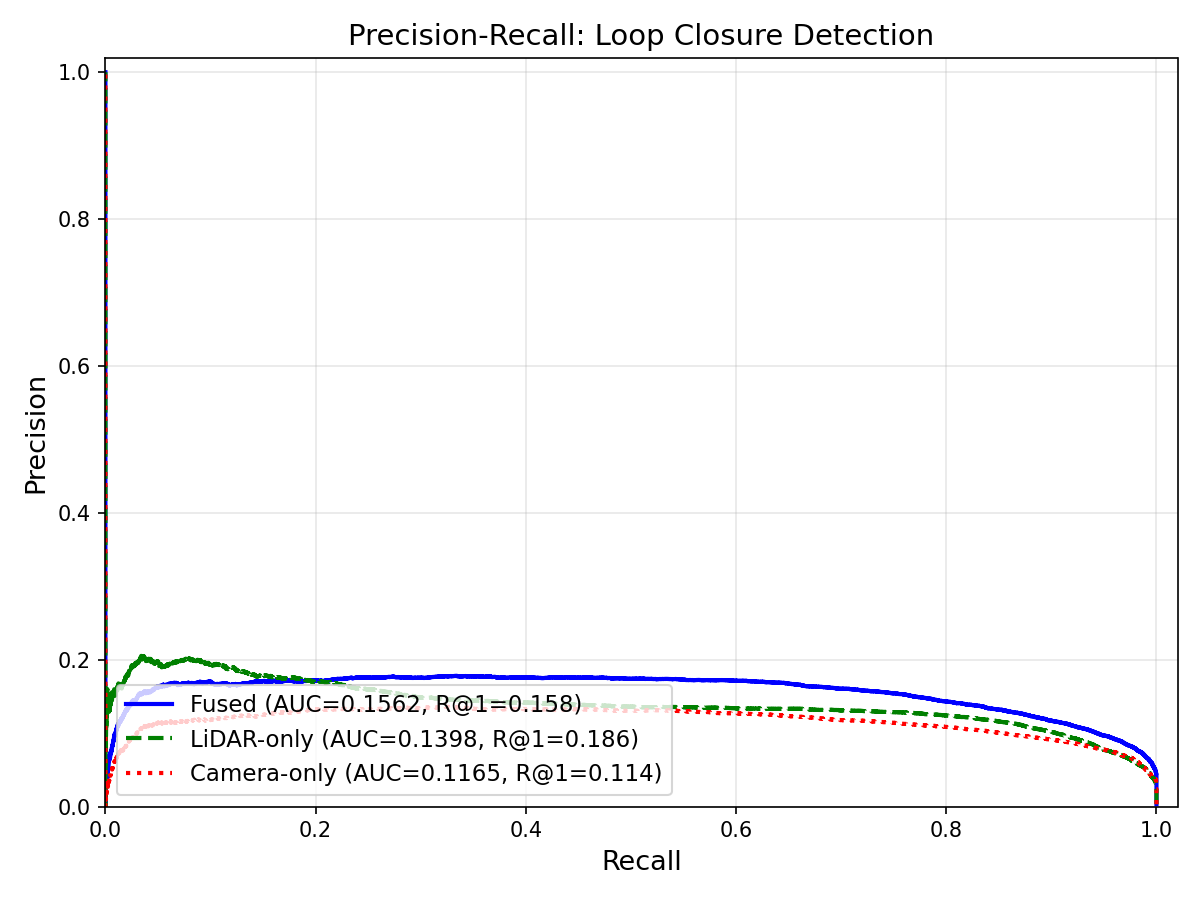
\includegraphics[width=0.85\linewidth]{figures/pr_curves.png}
    \caption{Precision-Recall curves for loop closure detection. The fused model (blue) achieves the highest AUC-PR (0.1562), outperforming LiDAR-only (green, 0.1398) and camera-only (red, 0.1165) baselines, demonstrating the benefit of multi-modal fusion.}
    \label{fig:pr_curves}
\end{figure}

\subsection{Analysis}

The fused descriptor consistently achieves the highest AUC-PR (0.1562) and F1-max (0.2675), validating our hypothesis that multi-modal fusion provides more discriminative location fingerprints than either modality alone. Notably:

\begin{itemize}
    \item \textbf{Fusion benefit:} The fused model improves AUC-PR by 11.7\% over LiDAR-only and 34.1\% over camera-only, demonstrating effective complementary information extraction.
    \item \textbf{LiDAR dominance at low recall:} LiDAR-only achieves higher Recall@1 (0.1864 vs.\ 0.1583), suggesting that geometric structure provides strong initial matching for the nearest neighbor. However, the fused model maintains higher precision at higher recall levels.
    \item \textbf{Modality dropout:} The ability to evaluate in single-modality mode (without retraining) is enabled by our modality dropout strategy during training.
\end{itemize}

\subsection{Limitations \& Planned Improvements}

While the current results demonstrate the viability of multi-modal fusion for loop closure, the absolute AUC-PR of 0.156 indicates significant room for improvement. We identify the following causes and planned next steps:

\begin{enumerate}
    \item \textbf{Harder Negative Mining:} The current negative distance threshold ($d_{\text{neg}} = 25$~m) produces negatives that are too easily distinguishable. We plan to reduce this threshold and implement semi-hard negative mining to focus training on the confusable distance band (25--50~m).
    
    \item \textbf{Larger Batch Sizes for Hard Mining:} With access to more compute, we will increase the PK batch sampler to $P{=}24$, $K{=}4$ (96 frames per batch), providing richer negative diversity during the hard mining phase.
    
    \item \textbf{Higher Embedding Dimensionality:} Increasing from 256-d to 512-d embeddings to provide the model more capacity for encoding fine-grained spatial distinctions.
    
    \item \textbf{Temporal Aggregation:} Extending the architecture with an LSTM or Temporal Convolutional Network (TCN) that processes a sliding window of $T$ consecutive frames, enabling the model to leverage sequential scene evolution rather than single-frame snapshots. This is expected to significantly reduce perceptual aliasing.
    
    \item \textbf{Multi-session Training:} The current dataset contains a single traversal session. Acquiring multi-session data (different times of day, weather conditions) would dramatically improve generalization.
\end{enumerate}

\section{Alignment with Course Syllabus}
\label{sec:alignment}

This project rigorously applies core concepts from COMP~841:
\begin{itemize}
    \item \emph{Convolutional Neural Networks (CNNs):} Applied in a two-stream architecture with ResNet-18 backbones for simultaneous spatial and visual feature extraction.
    \item \emph{Dimensionality Reduction:} Utilizing a bottleneck fusion MLP to compress 1024-d multi-modal features into a compact 256-d latent embedding.
    \item \emph{Optimization and Loss:} Implementation of Adam optimization with learning rate scheduling, and Triplet Margin Loss for metric learning with online batch-hard mining.
    \item \emph{Regularization:} Modality dropout, standard dropout, data augmentation, and Batch Normalization to prevent overfitting.
    \item \emph{Deep Neural Networks:} End-to-end training of a 23M-parameter multi-input descriptor generation pipeline with mixed precision and gradient accumulation.
\end{itemize}

\section{Expected Deliverables}
\label{sec:deliverables}

By the conclusion of the semester, we will deliver:
\begin{enumerate}
    \item A pre-processing pipeline leveraging ROS \texttt{message\_filters} to synchronize, project, and extract Ouster OS1-128 and RGB camera data from the 500+ GB dataset.
    \item A trained PyTorch multi-modal Siamese network capable of generating fused location descriptors, with modality dropout for graceful single-sensor degradation.
    \item A comprehensive performance report containing Precision-Recall curves comparing fused, LiDAR-only, and camera-only descriptors, with analysis of the fusion benefit.
    \item An investigation of advanced training strategies (online hard negative mining, temporal aggregation) and their impact on loop closure accuracy.
\end{enumerate}
